
\subsection*{Example of a Vector Space}

%%%Insert this to get the typewriter font so it looks like a real movie script
{\ttfamily
\fontdimen2\font=0.4em
\fontdimen3\font=0.2em
\fontdimen4\font=0.1em
\fontdimen7\font=0.1em
\hyphenchar\font=`\-


%%%%put a hypertarget around the opening bit of text
\hypertarget{scripts_vector_spaces_example}{This video talks about the} definition  of
a vector space. Even though the defintion looks long, complicated and abstract, it is actually
designed to model a very wide range of real life situations. As an example, consider the vector space
\[
V=\{\text{all possible ways to hit a hockey puck}\}\, .
\]
The different ways of hitting a hockey puck can all be considered as vectors. You can think about adding vectors
by having two players hitting the puck at the same time. This picture shows vectors $N$ and $J$ corresponding to the 
ways Nicole Darwitz and Jenny Potter hit a hockey puck, plus the vector obtained when they hit the puck together.
\begin{center}
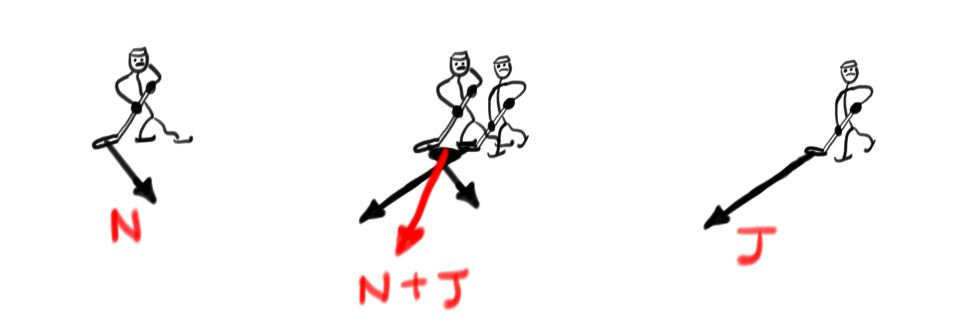
\includegraphics[alt={Nicole hits the hockey puck in direction N.  Nicole and Jenny hit it in direction N+J.  Jenny hits it in direction J.},scale=.35]{hockey.jpg}
\end{center}
You can also model the new  vector $2J$ obtained by scalar multiplication by $2$ by thinking about Jenny hitting the puck twice
(or a world with two Jenny Potters....). Now ask yourself questions like whether the multiplicative distributive law
\[2J + 2N = 2(J+N)\]
make sense in this context.





%%%%don't forget to close the bracket so the stuff after your file doesn't look like a movie!
}

%\newpage
